\chapter{Stand der Wissenschaft und Auswahl von Verfahren}

In diesem Kapitel soll der aktuelle Stand der Wissenscahft bezogen auf die in dieser Arbeit verwendeten Klassen von Verfahren betrachtet werden sowie ausgehend von den Anforderungen an das zu entwickelnde System ein passendes Verfahren ausgewählt und im Detail beschrieben werden. An geeigneten Stellen wird auf die im letztten Kapitel dargelegten Grundlagen zurückgegriffen.

\label{cha_state}

\section{SIEM-Systeme}

\label{sec_state_siem}

Zur Zeit gibt es eine vielfältige Auswahl an SIEM-Systemen auf dem Markt: Splunk\footnote{
  https://www.splunk.com
}, QRadar von IBM\footnote{
  https://www.ibm.com/us-en/marketplace/ibm-qradar-siem
} oder ArcSight von Micro Focus\footnote{
  https://software.microfocus.com/en-us/software/siem-security-information-event-management
} sind nur einige Beispiele aus diesem Bereich. Neben den in Abschnitt \ref{sec_basics_siem} beschriebenen grundlegenden Funktionen eines SIEM-Systems, die von allen Kandidaten in unterschiedlichem Maße bereitgestellt werden, unterscheiden sie sich insbesondere in darüber hinausgehenden Techniken: Die Nutzung von Machine Learning zur Erkennung ungewöhnlichem Verhaltens oder die Automatisierung von Handlungen im Bedrohungsfall sind hier beispielhafte Möglichkeiten.

Die Auswahl an quelloffener Software in diesem Bereich ist jedoch sehr gering. Eine Ausnahme stellt OSSIM - ein SIEM-System der Firma AlienVault\footnote{
	AlienVault OSSIM: The World’s Most Widely Used Open Source SIEM\\https://www.alienvault.com/products/ossim
} - dar, das auf Basis weiterer quelloffener Lösungen aus dem Netzwerksicherheits-Bereich unter anderem die in Abschnitt \ref{sec_basics_siem} beschriebenen Funktionen bereitstellt. AlienVault bietet zusätzliche eine kommerzielle Variante seines Produkts namens USM an, das insbesondere in den Bereichen Event-Korrelation und Compliance-Reporting die Funktionalität von OSSIM übersteigt. Von der Entwicklungsarbeit die in USM fließt, profitiert jedoch auch OSSIM, beispielsweise durch die Aktualisierung von Plugins für die Einbindung von aktuellen Netzwerkgeräten.

Da die Quelloffenheit auch die Möglichkeit bietet, Komponenten des SIEM-Systems direkt zu verändern, und außerdem gerade im Sicherheitsbereich generell zu bevorzugen ist, fiel die Entscheidung des in dieser Arbeit verwendeten SIEM-Systems auf OSSIM.

\subsection{OSSIM-Überblick}

\label{subsec_state_siem_overview}

Im Folgenden soll eine Übersicht über die für diese Arbeit relevanten Komponenten von OSSIM und deren Zusammenspiel gegeben werden. Diese ist auch in Abbildung \ref{fig:ossim_log_flow} dargestellt.

Den Kern des SIEM-Systems bildet der OSSIM-Server. Hier werden Events gespeichert sowie aggregiert und es findet die Korrelation von Events statt, die der Erkennung von Angriffen oder ungewöhnlichem Netzverhalten dient. Events und generierte Meldungen können über ein Web Interface betrachtet werden. Weiterhin können hier unter anderem Angaben zur Netzinfrastruktur bereitgestellt, Netzwerk- und Schwachstellenscanner bedient und sämtliche Informationen über den Netzwerkstatus eingesehen werden. 

Der OSSIM-Agent ist dafür zuständig, vorliegende Logdaten zu parsen und in ein OSSIM-spezifisches Event-Format zu übersetzen. Auf diesen Vorgang wird im nächsten Abschnitt genauer eingegangen. Die erzeugten Events werden anschließend an den Server weitergeleitet. Der Agent befindet sich sowohl direkt auf dem Server als auch auf jedem installierten Sensor. 

Eine OSSIM-Umgebung kann optional ein oder mehrere Sensoren nutzen, auf denen jeweils ein Agent seine Arbeit verrichtet. Dies wird im Folgenden verteilte Installation genannt. Der Vorteil dieser Lösung besteht darin, dass das aufwendige Parsen und Normalisieren von Logdaten verteilt staffinden und dadurch die Serverlast in großen Umgebungen reduziert werden kann. Kommt kein externer Sensor zum Einsatz, so spricht man von einer All-In-One-Installation.

\begin{figure}[]
    \centering
        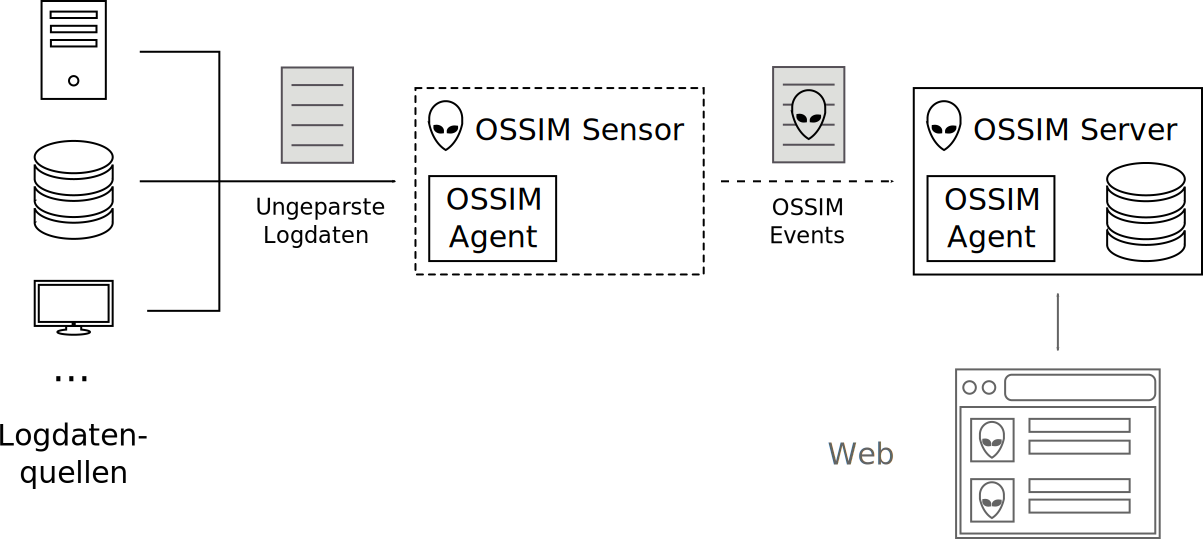
\includegraphics[width=0.9\textwidth]{dia/ossim_log_flow.pdf}
    \caption{High-Level-Übersicht über die OSSIM-Architektur und den Datenfluss.}
    \label{fig:ossim_log_flow}
\end{figure}


\subsection{Parsen von Logdaten in OSSIM}

\label{subsec_state_siem_parsing}

% Quellenarten
% Plugins
% OSSIM-Events
Besonders von Bedeutung für diese Arbeit ist die Verarbeitung von Logdaten. OSSIM ermöglicht es, Logdaten aus unterschiedlichen Quellen entgegenzunehmen bzw. aktiv selber abzurufen und in ein gemeinsames Event-Format zu übersetzen. Hierzu stehen verschiedene Möglichkeiten zur Verfügung:

\begin{itemize}
  \item Entgegennehmen von Daten über das Syslog-Protokoll
  \item Beschaffen von Daten über das SNMP-Protokoll
  \item Entgegennehmen von Daten über proprietäre Protokoll wie SDEE oder WMI
  \item Beschaffen von Daten durch Datenbankabfragen 
\end{itemize}

Unabhängig von der Datenquelle funktioniert die Verarbeitung der Logdaten nach dem immer gleichen Schema. OSSIM bietet die Möglichkeit mitgelieferte oder selber entwickelte Plugins für verschiedene Datenquellen zu aktivieren. Für eintreffende Logdaten überprüft der Agent anhand von regulären Audrücken, ob ein Plugin für das entsprechende Datum zuständig ist. Ist so ein Plugin gefunden, so wird ein neues OSSIM-Event angelegt und anhand der Angaben im Plugin die entsprechenden vorgegebenen Felder des Events gesetzt. Hierbei kann es sich beispielsweise um den Zeitpunkt des Events, IP-Adresse und Port der Datenquelle, einen zu dem Event gehörigen Netzwerkbenutzer oder ereignisabhängige selbstgesetzte Felder handeln. Anschließend folgt die Weiterleitung des Events an den Server.


\section{Pseudonymisierung}

\label{sec_state_pseudonymity}

- A name or another bit string. Identifiers, which are generated using random data only, i.e., fully 
independent of the subject and related attribute values, do not contain side information on the 
subject they are attached to, whereas non-random identifiers may do. E.g., nicknames chosen by 
a user may contain information on heroes he admires; a sequence number may contain 
information on the time the pseudonym was issued; an e-mail address or phone number contains 
information how to reach the user.  \cite{pfitzmann2010}

- evtl. Common Criteria

- VANET

- TIMSI

%pfitzmann2001 - Abschnitt 12
Der Begriff der Pseudonymisierung beschreibt die Benutzung von Pseudonymen zur Identifizierung von Subjekten. Pseudonymisierung sagt dabei erst einmal lediglich etwas über die Verwendung eines Verfahrens aus, jedoch nichts über die daraus entstehenden Auswirkungen auf die Identifizierbarkeit eines Subjekts oder die Zurechenbarkeit bestimmter Aktionen. Hierfür spielen weitere Eigenschaften von Pseudonymen wie die folgenden eine Rolle:
\begin{itemize}
  \item garantierte Eindeutigkeit von Pseudonymen
  \item Möglichkeit von Pseudonymänderungen
  \item begrenzt häufige Verwendung von Pseudonymen 
  \item zeitlich begrenzte Verwendung von Pseudonymen
  \item Art der Pseudonymserstellung
\end{itemize}

Die Ausprägungen dieser Eigenschaften werden auch im Rahmen dieser Arbeit für das umzusetzende System zu bewerten sein.

\section{Schwellwertschemata}

\begin{itemize}
  \item \textbf{Grundlagen} Von Shamirs Secret Sharing bis heute
  \item \textbf{Konkretes Verfahren} Im Detail erläutern - vmtl. Desmedt auf Basis von ElGamal
  \item Zusätzlich Erweiterungen dieses Verfahrens wie verteilte Schlüsselgenerierung.
\end{itemize}

%- Desmedt, Frankel: ElGamal \cite{DesmedtFrankel1990}
%- setzt zentralen "Dealer" voraus
%- Pedersen und verbesserte Variante 
%- Andere Möglichkeiten: Paillier, RSA, ...

\label{sec_state_threshold}

Ein solches System, das auf dem ElGamal-Algorithmus und damit dem Diskreten-Logarithmus-Problem basiert, veröffentlichten die Autoren in \cite{DesmedtFrankel1990}. \todo{Details} Dieser Ansatz setzt in der \textit{Setup}-Phase auf eine zentrale vertrauenswürdige Stelle zur Erzeugung der Schlüssel und \textit{Shares}. In \cite{pedersen1991} stellt der Autor basierend auf diesen Ergebnissen ein Verfahren vor, das bei der Schlüsselgenerierung ohne eine vertrauenswürdige Instanz auskommt. Dieses Verfahren wird in \cite{gennaro1999} noch einmal verbessert.\\
Basierend auf dem jetzigen Recherchestand würde sich diese Kombination von Verfahren gut für den angestrebten Anwendungszweck eignen. Konkrete offene Implementierungen wurden jedoch bisher nicht gefunden, so dass möglicherweise eine eigene Implementierung umgesetzt werden muss.

Neben diesem Verfahren gibt es noch weitere Ansätze basierend auf RSA \cite{desmedt1993, nguyen2005} oder dem Paillier-Kryptosystem \cite{paillier1999, damgard2001}, die jedoch deutlich komplexer zu sein scheinen. 

\todo{TBW}

\section{Searchable Encryption}

\todo{To be written...}